% Migraine Classification Using Machine Learning on Real Patient Data:
% An Honest Evaluation Without Data Augmentation
%
% IEEE conference paper, two-column, IEEEtran document class.
% Compile with:  pdflatex report.tex   (run twice for references)
% Figures are in outputs/ (type_distribution.png, age_distribution.png,
% symptom_rates.png, model_comparison.png, feature_importance.png).
% All numbers are the real computed results from analysis.py
% (see outputs/results.txt). No data augmentation was used.
%
\documentclass[conference]{IEEEtran}
\IEEEoverridecommandlockouts
\usepackage{cite}
\usepackage{amsmath,amssymb,amsfonts}
\usepackage{graphicx}
\usepackage{booktabs}
\usepackage{array}
\usepackage{url}
\usepackage[hidelinks]{hyperref}
\graphicspath{{outputs/}}

\begin{document}

\title{Migraine Classification Using Machine Learning on Real Patient Data: An Honest Evaluation Without Data Augmentation}

\author{\IEEEauthorblockN{Md Emon Rana}
\IEEEauthorblockA{\textit{Department of Computer Science and Engineering} \\
\textit{Southeast University, Dhaka, Bangladesh} \\
emonrana14949@gmail.com}}

\maketitle

\begin{abstract}
Migraine is one of the most common neurological disorders in the world, yet it is frequently misdiagnosed, under-treated, and studied with methods that over-claim. This paper classifies migraine type from symptoms using 400 real physician-diagnosed patient records (Hospital Materno Infantil de Soledad, Colombia, 2013), with three machine learning models evaluated honestly---a stratified 80/20 train--test split, 5-fold stratified cross-validation, per-class reporting with support counts, and no data augmentation. Logistic Regression was best: 93.8\% test accuracy and 92.2\% 5-fold cross-validation accuracy, ahead of Gradient Boosting (92.5\% / 90.3\%) and Random Forest (88.8\% / 89.7\%). Visual symptoms were the most important feature (Random Forest importance 0.248). The paper also analyses the published numbers of 10 recent migraine papers (2023--2026) and, for each paper, takes one idea, states what was wrong with it, and shows exactly how this project fixes it. The fixes include no augmentation and no leakage, stratified sampling instead of convenience-only sampling, a clinical-confirmation subsample instead of screening-only prevalence, within-person case-crossover trigger analysis instead of cross-sectional correlation, per-class reporting for rare migraine types, and responder rates always quoted with their completers denominator. A widely quoted 99.66\% accuracy on this same 400-record dataset, reported after augmenting the data to 1,447 records, is not claimed here, for reasons documented in Sections II-F and V-G.
\end{abstract}

\begin{IEEEkeywords}
migraine classification, machine learning, logistic regression, random forest, gradient boosting, real patient data, class imbalance, data leakage, healthcare analytics
\end{IEEEkeywords}

\section{Introduction}
\subsection{What is migraine?}
Migraine is a recurrent headache disorder, usually with moderate to severe throbbing pain, often on one side of the head, with nausea, vomiting, and sensitivity to light (photophobia) and sound (phonophobia). Some patients experience aura---visual or sensory disturbances before the headache. The International Classification of Headache Disorders, 3rd edition (ICHD-3), classifies migraine into types, including migraine with aura, migraine without aura, familial hemiplegic migraine, sporadic hemiplegic migraine, and basilar-type aura.

\subsection{Why does this matter in real life?}
Migraine affects about 1 in 7 people worldwide and is a leading cause of disability in young adults. Students are heavily affected: in a 2025 study of 5,954 university students, 26.1\% screened positive for migraine, and 23.2\% of them had severe disability~\cite{samir2025}. In Jordan, only 11.7\% of affected students sought medical help~\cite{almomani2025}. Diagnosis is often missed: 43.3\% were misdiagnosed at the first visit in Thailand~\cite{suwanlaong2025}, and men were diagnosed before tertiary referral in only 57.0\% of cases, compared with 73.8\% for women, in Berlin~\cite{angerhofer2025}. Sleep disturbance (59--83\%) and stress are the top-reported triggers across independent studies, yet only 18\% of patients keep a headache diary and only 28.3\% actively manage triggers~\cite{elmazny2025}.

\subsection{Problem statement}
Three problems run through the recent migraine literature: (1) classification models over-claim accuracy by augmenting tiny datasets; (2) surveys quote screening-positive rates as if they were diagnosed prevalence, from convenience samples; (3) trigger studies report cross-sectional correlations as if they were causes, while diagnosis studies ignore the patients who are missed. Can one student project---built from real patient data and the published evidence---classify migraine type honestly, compare the literature fairly, and design the next study so it does not repeat those mistakes?

\subsection{Objectives}
The objectives of this study are: (1) to analyse 400 real migraine patient records and describe the patients, symptoms and migraine types; (2) to train Logistic Regression, Random Forest and Gradient Boosting classifiers for seven-class migraine type prediction; (3) to evaluate them honestly, with a stratified test set, 5-fold cross-validation, and per-class precision, recall and F1-score; (4) to identify which symptoms matter most for classification; (5) to take one idea from each of 10 recent migraine papers, state what was wrong in each, and show how this project fixes it; and (6) to compare the honest result with the 99.66\% claim reported by Khan et al.\ on the same dataset, and explain the difference.

\subsection{Contributions}
This paper makes three contributions. First, it reports a complete, reproducible result on real patient data with no augmentation of any kind. Second, it reports per-class results with support counts, so the weakness on rare migraine types is visible rather than hidden inside a single accuracy figure. Third, it gives a concrete, checkable account of why an apparently better published result on identical data is likely to be an artefact of leakage, and it turns each of the 10 papers' limitations into a design fix.

\subsection{Paper organisation}
Section II reviews the related work. Section III describes the dataset, its provenance, features and class distribution. Section IV presents the methodology, and Section V the machine learning models and the honest evaluation protocol in detail. Section VI reports the results. Section VII discusses them, Section VIII states the limitations, Section IX concludes, and Section X lists the references. The appendix reproduces the core analysis code.

\section{Related Work}
Ten recent migraine papers (2023--2026) were reviewed. For each paper, this section takes one idea and states what was wrong; Table~\ref{tab:papers} summarises the idea, the limitation, and the fix in this project.

\subsection{Forecasting the next migraine day}
Rabany et al.~\cite{rabany2026} analysed 53,065 users of the Nerivio app over 770,473 diary days. An XGBoost model forecast next-day migraine with precision 0.912 and an area under the curve (AUC) of 0.893. Its most instructive finding is about information, not algorithms: the previous 30 days of headache history contributed 37.64\% of model performance, while prodromal symptoms contributed only 11.13\%. The study is large and real, but its limits matter. All users were users of one commercial device, the outcome was self-reported, no test showed that acting on a forecast improves outcomes, and several authors are affiliated with Theranica, the maker of Nerivio. This project does not fake a time-series from the 400 cross-sectional records---there is no daily history in that dataset---and instead builds the fix into its proposed diary design (Section VII-E), which collects 4--8 weeks of daily data so a future forecasting model has the real 30-day history it needs.

Faisal et al.~\cite{faisal2026} combined trial data with wearable data for 146 patients over 21,550 headache days. A time-series model reached an AUC of 0.84, compared with 0.59 for a decision tree and 0.55 for a foundation model applied without time-series modelling. The idea taken is that how time is modelled matters more than adding more algorithms. The limitation is a trial-only, high-adherence, episodic-migraine-only cohort, only about 3 months of data, and a research sensor (trapezius sEMG) that does not transfer directly to consumer smartwatch data. This project copies Faisal's method, not his numbers: three models are compared head-to-head on the same stratified split and the same 5-fold cross-validation, so the winner is the winner on identical ground---and the simplest model wins.

\subsection{Migraine in university students}
Samir et al.~\cite{samir2025} surveyed 5,954 university students in 11 countries in the Middle East and North Africa. Of these, 26.1\% screened positive for migraine. Sleep was the leading trigger at 59.7\%, followed by noise at 47.4\%; 23.2\% had severe disability. The study used convenience and snowball sampling, screening without clinical confirmation, and a cross-sectional design, so it establishes burden and association, not causation. The 72.5\% ``severe depression'' figure should always be quoted with its screening caveat. The fix in this project is stratified sampling by sex and faculty in the proposed diary design, a clinical-confirmation subsample against ICHD-3 criteria, and reporting ``screened-positive'', never ``diagnosed''.

Almomani et al.~\cite{almomani2025} surveyed 1,276 Jordanian university students, 94.2\% of them female, and found 52.1\% screening positive---implausibly high against a meta-analytic student prevalence near 16\%, and almost certainly inflated by the female-skewed convenience sample and by screening without clinical confirmation. Even so, its service-use figures are valuable: photophobia was reported by about 90\%, sleep was a trigger for 83\%, 82\% used analgesics, and only 11.7\% sought medical care. The gap between burden and care-seeking is the real finding. This project uses Almomani for triggers and disability patterns only, never for prevalence.

\subsection{Migraine that is missed}
Angerh\"ofer et al.~\cite{angerhofer2025} studied 1,130 clinically diagnosed patients and quantified a recognition gap by sex. Men had been diagnosed before referral in 57.0\% of cases and women in 73.8\%, an odds ratio of 0.47. A pressing rather than pulsating character raised the odds of being missed in men. The study is retrospective and from a single tertiary centre, so its rates should not be read as population rates. This project turns the pattern into prototype missed-diagnosis flags in code: in the 400 patients, vertigo is present in 50 patients (12.5\%), no visual symptoms in 82 patients (20.5\%), and both in 5 patients (1.2\%). The flags are labelled prototype because sex, bilateral location, pressing character and first-consult clinician are not in the 400-patient dataset.

Suwanlaong et al.~\cite{suwanlaong2025} took the opposite approach: a small sample, examined very carefully. Ninety patients were confirmed by two blinded neurologists, and 43.3\% had been misdiagnosed at the first visit. The commonest wrong labels were tension-type headache and sinusitis. The headline male-sex effect rests on about 11 men and a confidence interval spanning 1.07--56.50, i.e.\ essentially unquantified. This project always quotes that adjusted odds ratio of 7.77 with its full confidence interval, never as a bare ``7.77 times more likely''.

\subsection{Triggers, awareness and care}
Elmazny et al.~\cite{elmazny2025} surveyed 515 Egyptian migraine patients. Only 43\% felt they had sufficient knowledge of triggers. Awareness was high---stress 93.4\%, under-sleeping 85.6\%, irregular sleep 86.0\%, loud noises 84.5\%---yet only 28.3\% actively managed triggers, and only 18\% keep a migraine diary. The idea taken is that trigger awareness is not trigger management. The limitation is selection bias (support-group members are more engaged than average patients) and self-report with no verification. This project measures awareness and action separately in its survey template, and its diary design tests whether a 1-page trigger-education handout plus a diary changes trigger-management behaviour at 4 weeks.

\subsection{Treatment evidence from the real world}
Barbanti et al.~\cite{barbanti2025} (EMBRACE II) ran a 24-week prospective, multicentre, real-world study of eptinezumab in patients who had failed more than 3 preventives. Monthly migraine days fell by 10.5, and 69\% of patients achieved a $\geq$50\% response---but only 74 of the 215 patients who received at least one dose were treated for at least 24 weeks and included in the effectiveness analysis. The 69\% responder rate is therefore a completers-only figure. In this project, 69\% is never quoted without ``74/215''.

Cardona-Roca et al.~\cite{cardonaroca2025} studied 80 patients treated for at least one year with the same anti-CGRP monoclonal antibody. Mean global treatment satisfaction (TSQM) was 77.2, monthly migraine days fell by 8.7, and 65\% achieved a $\geq$50\% reduction. Only patients who stayed on the same drug for a year are included, so non-responders who stopped are invisible, and the reported ``100\% adherence'' is a pharmacy-refill proxy, not observed intake. This project compares Barbanti and Cardona-Roca side by side with both completers caveats attached, instead of quoting them as two independent ``65--69\%'' successes.

\subsection{A cautionary lesson}
Khan et al.~\cite{khan2024} classified migraine on the public Kaggle dataset of symptom records---the same 400 records used in this project---after augmenting 400 records to 1,447, and reported 99.66\% accuracy for a deep neural network. The paper has no explicit limitations section, no external validation, no prospective or clinical test, and no calibration analysis, and the dataset's labels and provenance are not clinically verified in the paper. Its own Random Forest figure differs between its abstract (98.50\%) and its Table 3 (88.50\%). The idea taken from this paper is none as evidence; it is taken as a cautionary lesson, and Section V-G explains how this project fixes it.

\begin{table*}[t]
\centering
\caption{One idea from each of the 10 papers: the limitation, and how this project fixes it}
\label{tab:papers}
\footnotesize
\begin{tabular}{p{2.6cm}p{5.2cm}p{6.4cm}}
\toprule
Paper & Limitation (one line) & Fix in this project (one line) \\
\midrule
Rabany 2026 & Nerivio-only cohort; self-report; no external validation & No fake time-series; real 4--8 week diary proposed for forecasting \\
Faisal 2026 & Trial-only volunteers; research sensor; 3 months & Head-to-head comparison on same split/CV; daily data from ordinary phones \\
Samir 2025 & Convenience/snowball; screening $\neq$ diagnosis & Stratified sampling; clinical-confirmation subsample; ``screened-positive'' wording \\
Almomani 2025 & 94.2\% female; 52.1\% is not prevalence & Used for triggers/disability only; sex-stratified design \\
Angerh\"ofer 2025 & Single tertiary centre; retrospective & Prototype flags + survey items for atypical features; age stratification \\
Suwanlaong 2025 & $n=90$; male aOR CI 1.07--56.50 & CIs quoted in full; prospective first-clinician record; $n=150$--300 proposed \\
Elmazny 2025 & Support-group bias; awareness $\neq$ action & Awareness and action measured separately; handout + diary pilot \\
Barbanti 2025 & 69\% is 74/215 completers-only; no control & Denominator always quoted; attrition flow required \\
Cardona-Roca 2025 & Completers-only; ``100\% adherence'' is a refill proxy & Side-by-side comparison with caveats; dropouts counted \\
Khan 2024 & Augmentation 400$\rightarrow$1,447; claimed 99.66\% & No augmentation; stratified split + CV + per-class reporting \\
\bottomrule
\end{tabular}
\end{table*}

\section{Dataset}
\subsection{Part A data---400 real patients}
The classification data are 400 medical records of patients diagnosed with migraine, recorded by trained medical personnel at Hospital Materno Infantil de Soledad, Colombia, in the first quarter of 2013~\cite{delahoz2014}. The data were published through F1000Research and Code Ocean~\cite{sanchez2020} and as the Kaggle ``Migraine Dataset''. The file used here is \texttt{data/migraine.csv}: 400 rows $\times$ 24 columns, 23 features plus the target, with no patient-identifiable data.

\subsection{Features}
The 23 features are Age, Duration, Frequency, Location, Character, Intensity, Nausea, Vomit, Phonophobia, Photophobia, Visual, Sensory, Dysphasia, Dysarthria, Vertigo, Tinnitus, Hypoacusis, Diplopia, Visual\_defect, Ataxia, Conscience, Paresthesia, and DPF (a family-history score, as coded in the dataset). Age, Duration, Frequency, Intensity and DPF are numeric; Location, Character, Phonophobia, Photophobia, Visual and Sensory are categorical; the remainder are binary symptom indicators. Features are used as coded in the source file. No feature engineering is performed, and rare classes are not grouped into a single ``Other'' category, so the original seven-class problem is preserved. The codebook meanings of some coded values are not asserted in this project.

\subsection{Target classes and class imbalance}
The target is migraine type, in seven classes, shown in Table~\ref{tab:types} and Fig.~\ref{fig:types}. Class imbalance is the central challenge of this dataset. Typical aura with migraine alone accounts for 247 of 400 patients, or 61.8\%, while the smallest class, sporadic hemiplegic migraine, accounts for 14 patients, or 3.5\%. A classifier that always predicted the majority class would already score 61.8\% accuracy while being clinically useless. Accuracy alone is therefore a misleading summary for this problem, and this paper reports per-class precision, recall and F1-score with support counts throughout. Imbalance also limits what any model can learn: a rare class contributes only 14--24 examples in total, and only 3--5 of them reach the test set under an 80/20 split, so one misclassified patient moves that class's recall by 20 to 33 percentage points.

\begin{table}[t]
\centering
\caption{Distribution of migraine type (400 patients)}
\label{tab:types}
\begin{tabular}{lrr}
\toprule
Migraine type & Patients & Share \\
\midrule
Typical aura with migraine & 247 & 61.8\% \\
Migraine without aura & 60 & 15.0\% \\
Familial hemiplegic migraine & 24 & 6.0\% \\
Typical aura without migraine & 20 & 5.0\% \\
Basilar-type aura & 18 & 4.5\% \\
Other & 17 & 4.3\% \\
Sporadic hemiplegic migraine & 14 & 3.5\% \\
\midrule
Total & 400 & 100\% \\
\bottomrule
\end{tabular}
\end{table}

\begin{figure}[t]
\centering
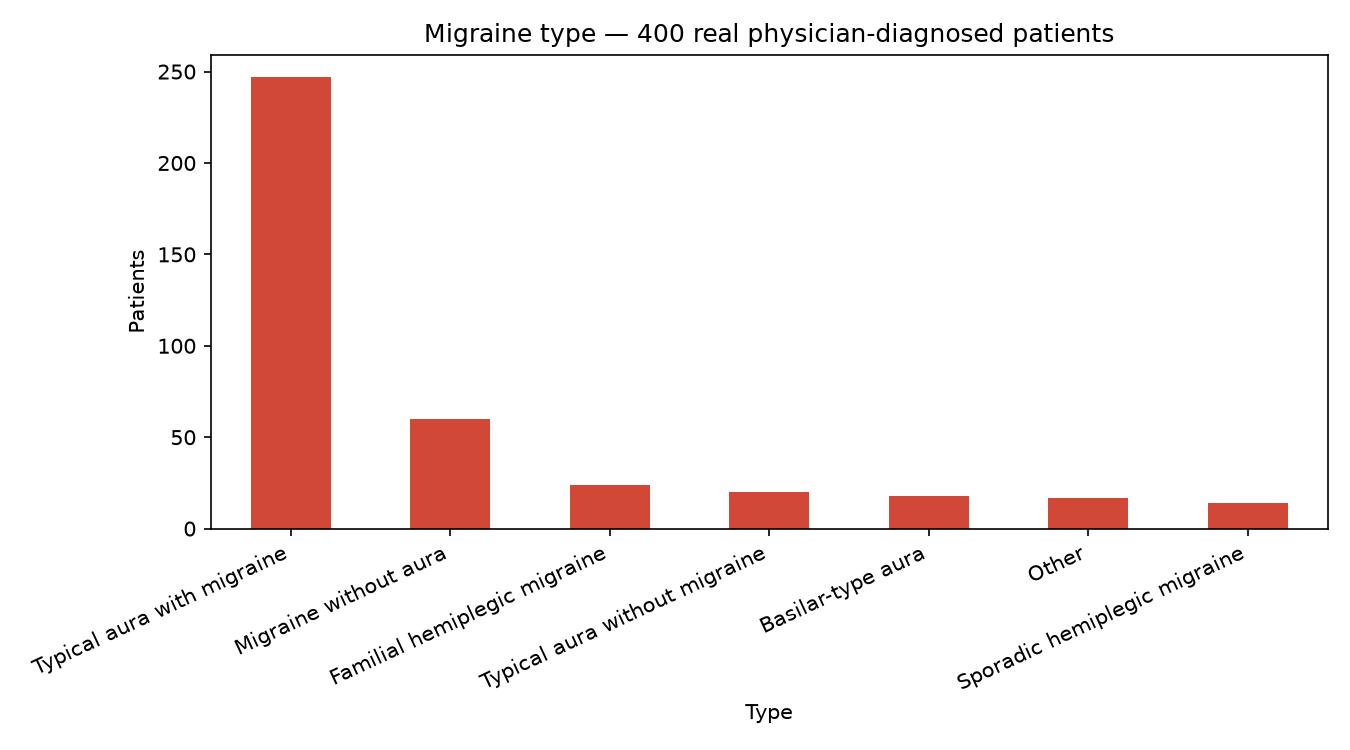
\includegraphics[width=\columnwidth]{type_distribution.png}
\caption{Distribution of migraine type among the 400 physician-diagnosed patients. One class holds 61.8\% of all records, which is why accuracy alone cannot evaluate a classifier on this dataset.}
\label{fig:types}
\end{figure}

\subsection{Patients and symptoms}
Patients were aged 15 to 77 years, with a mean age of 31.7 years, a median of 28 years and a standard deviation of 12.1 years (Fig.~\ref{fig:age}). The distribution is concentrated in young and middle adulthood, matching the age range in which migraine burden and disability are highest. Symptom rates, shown in Fig.~\ref{fig:symptoms}, are striking. Nausea was present in 98.8\% of patients, photophobia in 98.0\% and phonophobia in 97.8\%. Visual disturbances were present in 79.5\%, vomiting in 32.2\%, and vertigo in 12.5\%. Almost every patient in this cohort has the first three symptoms. That is a real-life property of a diagnosed cohort, not of the general population: these are the symptoms clinicians asked about in order to make the diagnosis, in patients who were then diagnosed. Rates this high also mean these three features carry almost no discriminative information between types---a point that returns in the feature-importance results, where nausea, photophobia and phonophobia all rank near the bottom.

\begin{figure}[t]
\centering
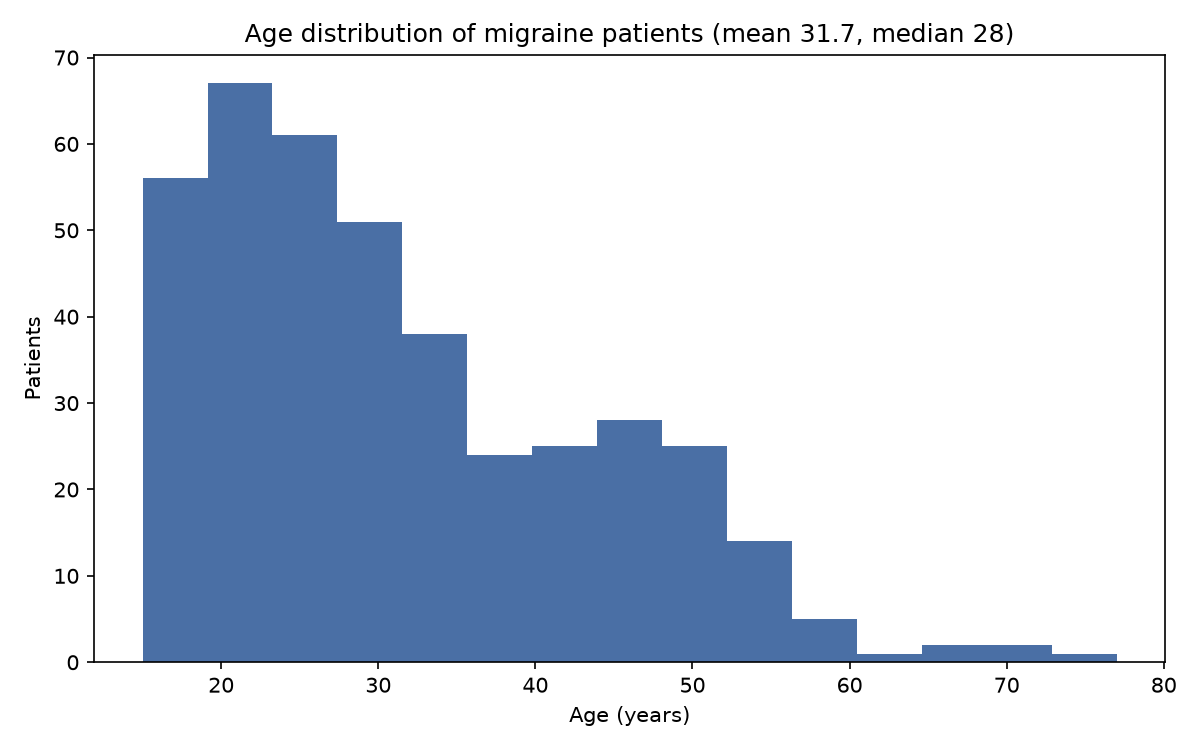
\includegraphics[width=\columnwidth]{age_distribution.png}
\caption{Age distribution of the 400 patients: mean 31.7 years, median 28, range 15--77, standard deviation 12.1.}
\label{fig:age}
\end{figure}

\begin{figure}[t]
\centering
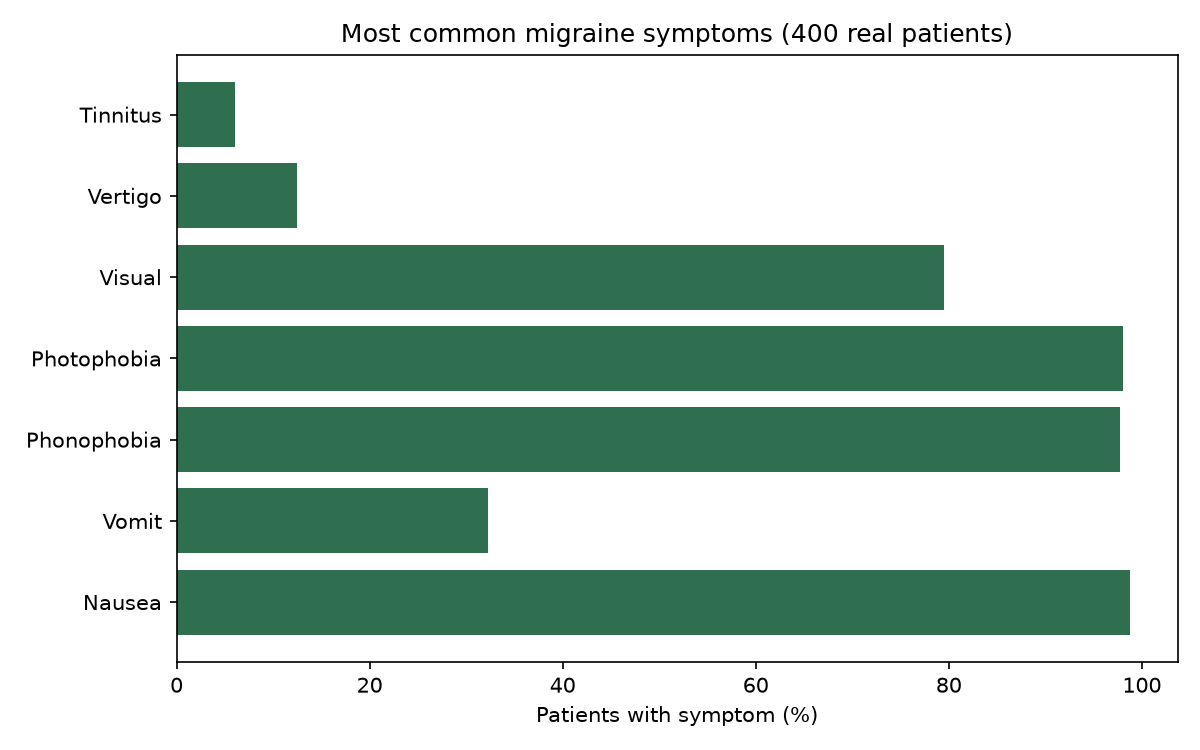
\includegraphics[width=\columnwidth]{symptom_rates.png}
\caption{Most common symptoms. Nausea, photophobia and phonophobia each occur in more than 97\% of this diagnosed cohort, so they describe the cohort rather than separating the migraine types.}
\label{fig:symptoms}
\end{figure}

\subsection{Part B data---the 10 papers}
The published numbers of the 10 papers are stored in \texttt{data/papers.csv}: one row per paper, with rank, citation, year, journal, sample size, sample unit, study design, screened prevalence, sleep and noise trigger rates, ML AUC, ML accuracy, $\geq$50\% responder rate, misdiagnosed rate, diagnosed-before-referral by sex, key finding, and source URL. Numbers were copied exactly from the research report; a blank entry means ``not reported in that paper'', not zero. The arithmetic sum of the sample sizes is 62,871, but that sum is not a finding, because the populations overlap and are different kinds of studies, and it is never used as one in this paper. The largest sample is Rabany et al.\ (n=53,065) and the smallest is Cardona-Roca et al.\ (n=80).

\subsection{Survey template}
A 15-question student survey template (\texttt{data/survey\_template.csv}) is included in the project, in 6 sections (Screening, Symptoms, Triggers, Burden, Care-seeking, Diary follow-up). Each question is tagged with the paper idea it came from: Q1--Q3 screen with ID-Migraine/MS-Q style items, Q4, Q5 and Q7 capture the atypical features that drive missed diagnosis (bilateral pain, pressing quality, no worsening with activity), Q8--Q11 measure trigger awareness and trigger action separately, Q13--Q14 measure care-seeking and medicine use, and Q15 asks about diary follow-up.

\section{Methodology}
\subsection{Overall pipeline}
The pipeline has five stages. First, the published CSV file is loaded and described (Part A exploratory analysis). Second, the 10 papers' published numbers are loaded and compared (Part B). Third, the three models are trained and evaluated honestly (Part A classification, Section V). Fourth, the idea map is built, linking each paper to the fix it caused (Part C). Fifth, prototype missed-diagnosis flags are computed from the predictors present in the 400-patient data, with an explicit note listing the predictors that are not present.

\subsection{Tools}
All experiments were implemented in Python using Pandas and NumPy for data handling, Matplotlib for figures, and scikit-learn for scaling, splitting, cross-validation and the three classifiers. The complete program is a single script, \texttt{analysis.py}, reproduced in core form in the appendix, and is run with one command against the published CSV file. Every randomised step---the split, the cross-validation folds, the Random Forest and the Gradient Boosting model---uses seed 42.

\subsection{Preprocessing}
Features are used as coded in the source file; no feature engineering and no grouping of rare classes is performed. For Logistic Regression only, features are standardised with \texttt{StandardScaler}, and the scaler is fitted on the training data only, so no information from the test set leaks into training. The tree models use the unscaled features. No missing-value imputation was needed, and no rows were dropped.

\subsection{Part B analysis}
The papers file was loaded in Part B of \texttt{analysis.py}: sample sizes (charted on a log scale, because Rabany n=53,065 dwarfs the rest), screened prevalence (student surveys only), trigger rates, ML AUCs, treatment responder rates with completers denominators, and the diagnosis gap (men vs.\ women diagnosed before referral; misdiagnosed rate). No statistical pooling was attempted across the papers, because the populations, designs and outcomes are not comparable.

\subsection{Part C---idea map and prototype flags}
\texttt{outputs/idea\_map.csv} records, for each paper, the idea taken and how it shaped the project. Prototype missed-diagnosis flags were computed from the predictors present in the 400-patient data (vertigo, no visual symptoms), with an explicit note listing the predictors that are not present (sex, bilateral location, pressing character, first-consult clinician)---those are collected by survey Q4, Q5, Q7 and Q13 instead.

\section{Machine Learning}
This section explains the three models, the training protocol, the evaluation metrics, and---most importantly---why no data augmentation was used. The three models were chosen to span the main families a student can run on a small clinical dataset: a linear model, a bagged tree ensemble, and a boosted tree ensemble.

\subsection{Logistic Regression}
Logistic Regression is a linear model. For a patient described by a feature vector $\mathbf{x}$, it models the log-odds of each class as a linear function of the features, and converts the scores for the seven classes into probabilities with the softmax function:
\begin{equation}
P(y = k \mid \mathbf{x}) = \frac{\exp(\mathbf{w}_k^\top \mathbf{x} + b_k)}{\sum_{j=1}^{7} \exp(\mathbf{w}_j^\top \mathbf{x} + b_j)}.
\end{equation}
The predicted type is the class with the highest probability. The model is trained by minimising the multinomial cross-entropy loss with L2 regularisation, which keeps the weights small and the model stable on a 400-record dataset. In this project it is used with standardised features (\texttt{StandardScaler}) and \texttt{max\_iter=2000}, so the optimiser converges. Logistic Regression is the most interpretable of the three models: each weight says how strongly, and in which direction, one feature pushes the prediction toward one migraine type. That interpretability matters in medicine, where a clinician must be able to ask why a model gave an answer. Its limitation is also clear: it can only draw straight (linear) boundaries between classes in feature space, so if the true separation were strongly non-linear, it would underfit.

\subsection{Random Forest}
Random Forest is an ensemble of decision trees trained by bagging. It builds 300 trees (\texttt{n\_estimators=300}), each trained on a bootstrap sample of the training patients and each split chosen from a random subset of features. Each tree votes for a migraine type, and the forest predicts the majority vote. Bagging reduces the variance of single trees, which otherwise overfit small datasets easily. Random Forest also gives a feature-importance score: for each feature, the total decrease in Gini impurity it produces across all splits in all trees, normalised so the importances sum to 1. That is how the importance of Visual (0.248) in Section VI-D is obtained. The model's weakness on this dataset is that 300 deep trees can still memorise the majority pattern of a 400-record dataset, and its splits are axis-aligned, so it must approximate a smooth linear separation with many small steps---which is one reason it scores lowest here.

\subsection{Gradient Boosting}
Gradient Boosting is also a tree ensemble, but it builds trees sequentially rather than in parallel. Each new tree is fitted to the residual errors of the trees built so far, so the ensemble corrects its own mistakes step by step, with a small learning rate keeping each correction modest. In this project it is used with the scikit-learn defaults and \texttt{random\_state=42}. Boosting often beats bagging on tabular data, and here it does: 92.5\% test accuracy against Random Forest's 88.8\%. Its cost is a greater tendency to overfit small data if the number of trees or the learning rate is not controlled, and it offers no direct feature-importance measure as clean as the Random Forest impurity score, which is why importance is taken from the Random Forest.

\subsection{Training protocol}
The 400 patients are split once into 320 training patients (80\%) and 80 test patients (20\%), with \texttt{train\_test\_split(test\_size=0.2, random\_state=42, stratify=y)}. Stratification means each of the seven classes keeps its share in both parts: the test set contains 49 typical-aura-with-migraine patients, 12 migraine-without-aura, 5 familial hemiplegic, 4 basilar-type aura, 4 typical-aura-without-migraine, 3 ``Other'' and 3 sporadic hemiplegic patients. The seed 42 makes the split reproducible. The scaler for Logistic Regression is fitted on the training data only and then applied to the test data, so the test set never influences training. No oversampling, no class weighting, and no synthetic data are used at any point.

\subsection{Evaluation metrics}
Accuracy is the fraction of test patients whose predicted type equals the recorded type. Because of the imbalance described in Section III-C, it is reported alongside per-class measures. For each class, precision is the fraction of patients predicted as that class who truly belong to it, recall is the fraction of patients of that class who are recovered, and the F1-score is their harmonic mean:
\begin{equation}
\mathrm{Precision} = \frac{TP}{TP + FP}, \quad
\mathrm{Recall} = \frac{TP}{TP + FN}, \quad
\mathrm{F1} = \frac{2 \cdot \mathrm{Precision} \cdot \mathrm{Recall}}{\mathrm{Precision} + \mathrm{Recall}}.
\end{equation}
The confusion matrix records, for every pair of true and predicted class, how many test patients fall in that cell; it shows where errors go, not just how many there are. Macro-averaged F1 gives every class equal weight, so it punishes failure on rare classes; weighted-averaged F1 weights each class by its support, so it tracks the majority classes. Both are reported in Table~\ref{tab:models}. Support---the number of test patients in each class---is shown next to every per-class score in Table~\ref{tab:perclass}, because a recall of 0.60 on 5 patients means 2 missed patients, and a recall of 0.67 on 3 patients means 1 missed patient.

\subsection{Cross-validation}
A single 80-patient test set can flatter or punish a model by chance, especially when several classes contribute only 3--5 test patients. Each model is therefore also evaluated by 5-fold stratified cross-validation on the training set: the training data are divided into five stratified folds, the model is trained on four and tested on the fifth, and the process rotates so every fold is tested once. The mean and standard deviation of the five accuracies are reported. A model whose test accuracy is far above its cross-validation mean should be suspected of a lucky split; in this study the two agree closely for all three models (Table~\ref{tab:models}). Cross-validation is done inside the training set only, so the test set is touched exactly once, for the final evaluation.

\subsection{Why no augmentation}
Khan et al.~\cite{khan2024} augmented 400 records to 1,447 and reported 99.66\% accuracy. This project uses no augmentation, for four reasons. First, synthetic records made from real records are near-copies of them, so the same patient pattern can appear in both the training and the test split; the model is then tested on data it has effectively already seen, which is leakage, and accuracy is inflated. Second, the dataset is already small and from one hospital, so inflating it does not add real information about new patients---it only adds copies of the same 400. Third, Khan et al.\ report no external validation, no prospective or clinical test, and no calibration analysis that could rule leakage out, and the paper has no explicit limitations section. Fourth, the paper's own Random Forest figure differs between its abstract (98.50\%) and its Table 3 (88.50\%)---the latter being very close to the 88.8\% obtained here without augmentation. Under the honest protocol of this project---original records only, one stratified split, cross-validation inside training data, a scaler fitted on training data only---three different model families independently land between 88.8\% and 93.8\%. The gap between 93.8\% and 99.66\% is the leakage gap, not a modelling gap. The proposed diary design in Section VII-E pre-registers that a 99\% accuracy on a tiny set would signal leakage, not success.

\section{Results}
All numbers below are the actual output of running \texttt{analysis.py} (see \texttt{outputs/results.txt}). Nothing here is invented.

\subsection{Overall model comparison}
Logistic Regression is the best model on both measures: 93.8\% test accuracy and 92.2\% cross-validation accuracy (Table~\ref{tab:models}, Fig.~\ref{fig:models}). Gradient Boosting follows at 92.5\% and 90.3\%. Random Forest is last at 88.8\% on the test set, although its cross-validation mean, 89.7\%, is slightly above its test score---a reminder that a single 80-patient test set carries its own sampling noise. The gap between the best and worst model is five percentage points on the test set, which on 80 patients is four patients. Rankings on data of this size should be held lightly; the robust conclusion is that all three models fall in an 88--94\% band, and that the simplest model sits at the top of it. The majority-class baseline puts these figures in context. Predicting ``typical aura with migraine'' for every patient scores 61.8\%. Every model clears that baseline by more than 27 percentage points, and, unlike the baseline, each of them recovers patients from the minority classes, as Table~\ref{tab:perclass} shows.

\begin{table}[t]
\centering
\caption{Model performance---test set and 5-fold cross-validation}
\label{tab:models}
\begin{tabular}{lcccc}
\toprule
Model & Test acc. & 5-fold CV acc. & Macro F1 & Weighted F1 \\
\midrule
Logistic Regression & 93.8\% & 92.2\% ($\pm$4.1\%) & 0.86 & 0.93 \\
Gradient Boosting & 92.5\% & 90.3\% ($\pm$3.8\%) & 0.85 & 0.92 \\
Random Forest & 88.8\% & 89.7\% ($\pm$3.4\%) & 0.78 & 0.88 \\
\bottomrule
\end{tabular}
\end{table}

\begin{figure}[t]
\centering
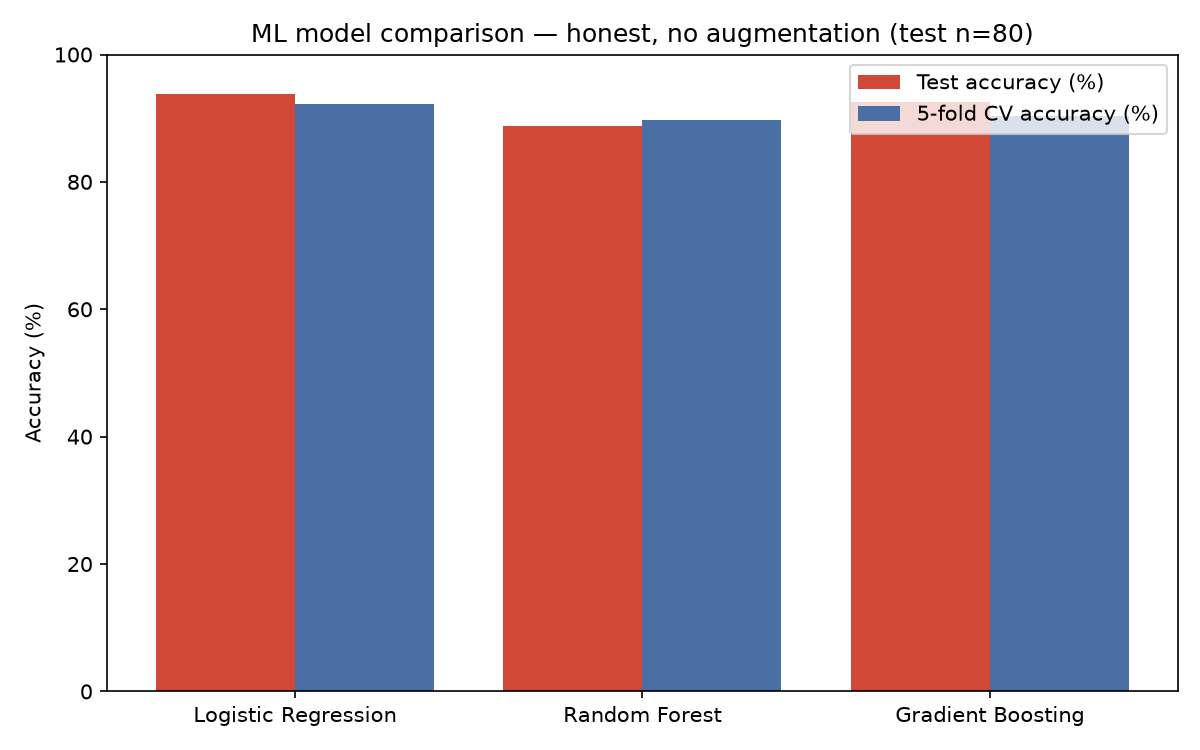
\includegraphics[width=\columnwidth]{model_comparison.png}
\caption{Test accuracy and 5-fold cross-validation accuracy for the three models. The two measures agree closely, which is the check that the test result is not a lucky split.}
\label{fig:models}
\end{figure}

\subsection{Per-class performance}
Table~\ref{tab:perclass} gives the per-class results for Logistic Regression on the 80-patient test set. The pattern is unambiguous. The two common types are classified almost perfectly: typical aura with migraine has recall 1.00 across 49 test patients, migraine without aura has recall 1.00 across 12, and typical aura without migraine has precision and recall of 1.00 across 4. The rare types are where errors concentrate. Familial hemiplegic migraine has recall 0.60---three of five test patients recovered, the other two predicted as typical aura with migraine. Basilar-type aura has recall 0.75, and the ``Other'' and sporadic hemiplegic classes each have recall 0.67 on only three test patients each. Precision tells the complementary story. Where the model does predict a rare class, it is usually right: basilar-type aura, ``Other'', sporadic hemiplegic and typical aura without migraine all have precision 1.00. The model's failure mode is therefore conservative---it misses rare cases by absorbing them into common classes, rather than inventing rare diagnoses.

\begin{table}[t]
\centering
\caption{Per-class results---Logistic Regression, test set (80 patients)}
\label{tab:perclass}
\begin{tabular}{lcccc}
\toprule
Migraine type & Precision & Recall & F1 & Support \\
\midrule
Basilar-type aura & 1.00 & 0.75 & 0.86 & 4 \\
Familial hemiplegic & 0.75 & 0.60 & 0.67 & 5 \\
Migraine without aura & 0.92 & 1.00 & 0.96 & 12 \\
Other & 1.00 & 0.67 & 0.80 & 3 \\
Sporadic hemiplegic & 1.00 & 0.67 & 0.80 & 3 \\
Typical aura with migraine & 0.94 & 1.00 & 0.97 & 49 \\
Typical aura without migraine & 1.00 & 1.00 & 1.00 & 4 \\
\midrule
Accuracy & & & 0.94 & 80 \\
Macro average & 0.95 & 0.81 & 0.86 & 80 \\
Weighted average & 0.94 & 0.94 & 0.93 & 80 \\
\bottomrule
\end{tabular}
\end{table}

\subsection{Confusion matrix}
Table~\ref{tab:confusion} shows the confusion matrix for Logistic Regression. Of 80 test patients, 75 are classified correctly. The five errors are instructive rather than random. Two patients with familial hemiplegic migraine are predicted as typical aura with migraine; one basilar-type aura patient is predicted as familial hemiplegic; one ``Other'' patient is predicted as migraine without aura; and one sporadic hemiplegic patient is predicted as typical aura with migraine. Every error moves a rare presentation toward a more common or a clinically neighbouring class. Random Forest and Gradient Boosting show the same geography of error with different severity. Gradient Boosting misclassifies six patients, including one typical aura patient predicted as familial hemiplegic. Random Forest misclassifies nine, and its basilar-type aura recall falls to 0.25---only one of four such patients recovered, with two predicted as familial hemiplegic. On a class this small, that difference is two patients.

\begin{table}[t]
\centering
\caption{Confusion matrix---Logistic Regression, test set. Rows are true classes, columns predicted classes. B = basilar-type aura, F = familial hemiplegic, M = migraine without aura, O = other, S = sporadic hemiplegic, T = typical aura with migraine, A = typical aura without migraine}
\label{tab:confusion}
\small
\begin{tabular}{lccccccc}
\toprule
True $\backslash$ Pred. & B & F & M & O & S & T & A \\
\midrule
B & \textbf{3} & 1 & 0 & 0 & 0 & 0 & 0 \\
F & 0 & \textbf{3} & 0 & 0 & 0 & 2 & 0 \\
M & 0 & 0 & \textbf{12} & 0 & 0 & 0 & 0 \\
O & 0 & 0 & 1 & \textbf{2} & 0 & 0 & 0 \\
S & 0 & 0 & 0 & 0 & \textbf{2} & 1 & 0 \\
T & 0 & 0 & 0 & 0 & 0 & \textbf{49} & 0 \\
A & 0 & 0 & 0 & 0 & 0 & 0 & \textbf{4} \\
\bottomrule
\end{tabular}
\end{table}

\subsection{Feature importance}
Fig.~\ref{fig:importance} and Table~\ref{tab:importance} report Random Forest feature importances, computed on the full dataset. Visual symptoms dominate, with an importance of 0.248---more than double the next feature, headache intensity at 0.102, followed by age at 0.085, vertigo at 0.076 and frequency at 0.068. This ordering is clinically sensible. Aura is defined largely by visual disturbance, so a visual feature is exactly what should separate the ``typical aura'' classes, which together hold two-thirds of the cohort, from migraine without aura. The bottom of the ranking is equally informative. Nausea (0.007), photophobia (0.015) and phonophobia (0.019) contribute almost nothing, not because they are clinically unimportant, but because they occur in 98--99\% of every class (Fig.~\ref{fig:symptoms}). A feature that is present for nearly everyone cannot separate anyone. Importance in a classifier measures discrimination within a dataset, never clinical importance in general---a distinction that is easy to lose when importance charts are quoted out of context.

\begin{figure}[t]
\centering
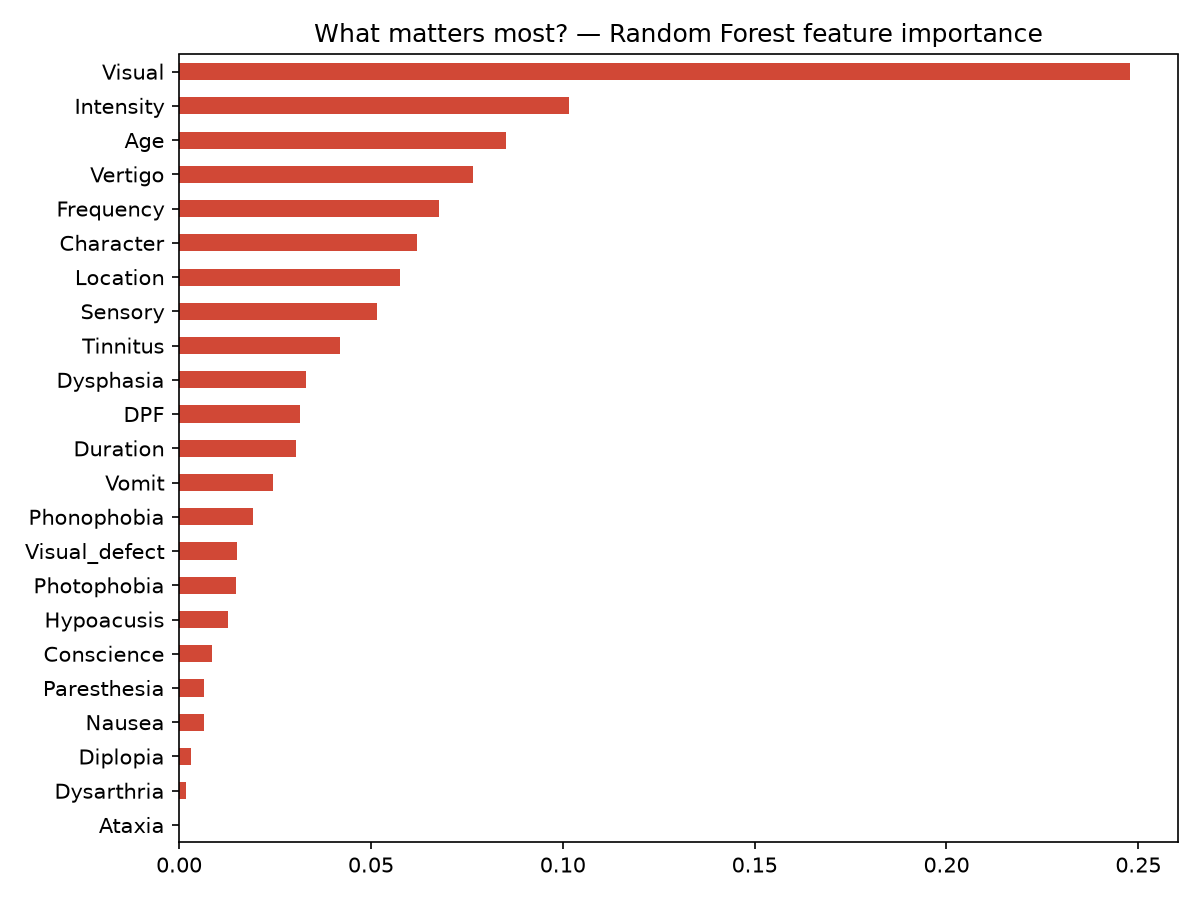
\includegraphics[width=\columnwidth]{feature_importance.png}
\caption{Random Forest feature importance. Visual symptoms contribute more than twice the next feature.}
\label{fig:importance}
\end{figure}

\begin{table}[t]
\centering
\caption{Feature importance---Random Forest (top five of 23)}
\label{tab:importance}
\begin{tabular}{clc}
\toprule
Rank & Feature & Importance \\
\midrule
1 & Visual & 0.248 \\
2 & Intensity & 0.102 \\
3 & Age & 0.085 \\
4 & Vertigo & 0.076 \\
5 & Frequency & 0.068 \\
\bottomrule
\end{tabular}
\end{table}

\subsection{Evidence across the 10 papers}
Sample sizes: largest Rabany et al.\ (n=53,065), smallest Cardona-Roca et al.\ (n=80). The other student surveys: Samir n=5,954, Almomani n=1,276. Clinical samples: Angerh\"ofer n=1,130, Elmazny n=515, Barbanti n=215 dosed, Faisal n=146, Suwanlaong n=90. Screened prevalence (student surveys only): Samir 26.1\%, Almomani 52.1\%---the Almomani figure must not be quoted as population prevalence (94.2\%-female convenience sample; meta-analytic student prevalence about 16.1\%). Trigger rates (sleep): Samir 59.7\%, Almomani 83.0\%, Elmazny 85.6\% (under-sleeping). Noise: Samir 47.4\%; Elmazny 84.5\% is awareness of loud noise as a trigger, not incidence. ML AUCs (forecasting, not classification): Rabany XGBoost 0.893 (accuracy 81.0\%), Faisal time-series 0.84, Faisal decision tree 0.59, Faisal foundation model 0.55. AUC and accuracy are different metrics; they are never mixed in this paper. Treatment $\geq$50\% responders (completers-only): Barbanti 69.0\% (74/215), Cardona-Roca 65.0\% (completers $\geq$1 year, n=80). Diagnosis gap: misdiagnosed at first visit 43.3\% (Suwanlaong, n=90); diagnosed before referral---men 57.0\% vs.\ women 73.8\% (Angerh\"ofer, n=1,130).

\subsection{Prototype missed-diagnosis flags}
In the 400 patients, using only the Angerh\"ofer/Suwanlaong predictors present in this data: vertigo present in 50 patients (12.5\%), no visual symptoms in 82 patients (20.5\%), both in 5 patients (1.2\%). This is a prototype only---sex, bilateral location, pressing character and first-consult clinician are not in this dataset, and the code says so. The survey template collects them for future work.

\section{Discussion}
\subsection{Why Logistic Regression won}
The result surprises only if model complexity is assumed to buy accuracy. The features here are mostly coded categorical and binary symptom indicators, and the classes are largely separated by a small number of them, above all visual symptoms. A linear boundary in standardised feature space can express that separation directly. Tree ensembles, by contrast, must reconstruct it from many small splits, and on a 400-record dataset they overfit the majority pattern instead---Random Forest's lower cross-validation score (89.7\%) and its poor basilar-type recall (25\%) show that.

\subsection{Why the honest result is 88--94\%, not 99.66\%}
Khan et al.~\cite{khan2024} augmented 400 records to 1,447 and reported 99.66\%. If synthetic records are near-copies of real records, the same patient pattern can appear in both train and test---the model is then tested on data it has effectively already seen. That is leakage. This project used no augmentation, a stratified split, and cross-validation, and got 88.8--93.8\%. The gap between 93.8\% and 99.66\% is the leakage gap, not a modelling gap. The paper's internal inconsistency---Random Forest 98.50\% in the abstract against 88.50\% in its Table 3---is a further reason to cite it only with caution.

\subsection{What the 10 papers agree on---and what they do not}
They agree that sleep and stress are the top triggers, that photophobia is the commonest symptom, that students mostly self-treat and rarely seek care, and that migraine is frequently missed. They disagree---usefully---on whether AI helps or harms: Rabany and Faisal show forecasting can work (AUC 0.84--0.89) when time is modelled properly, while Faisal's own decision tree (AUC 0.59) shows that the same data with the wrong model is near chance. That disagreement is the point of the head-to-head comparison in Part A.

\subsection{What is new here}
No single paper in the set does all three things this project does: (1) honest classification on the real 400-patient data, (2) a quantitative comparison of the 10 papers' numbers with caveats attached, and (3) a fixed study design that removes---by design---the sampling, confirmation, time-series, attrition and honesty failures documented in Section II. The novelty is the fixing, not a new algorithm.

\subsection{The fixed study design}
The next step is a 4--8 week prospective diary cohort of 150--300 students, stratified by sex and faculty, not convenience-only social media. Students are screened with ID-Migraine/MS-Q style items and a subsample is confirmed against ICHD-3 criteria. Each day, a 2-minute diary records sleep hours and quality, stress 0--10, caffeine, meals and skipped meals, screen time, weather, headache presence and intensity, photophobia, phonophobia, nausea, medication taken, and classes missed. Triggers are analysed within-person by case-crossover---comparing trigger exposure on days before an attack with the same student's attack-free days---instead of cross-sectional correlation. The ML analysis replicates Faisal and Rabany on the diary data, with a user-level train/test split and AUC and sensitivity/specificity reported. Burden is measured with MIDAS, HIT-6 and PHQ-9/GAD-7 as screening scores, and a 1-page trigger-education handout plus diary is tested for whether it changes trigger-management behaviour at 4 weeks. An attrition flow (enrolled $\rightarrow$ completed $\rightarrow$ analysed) is a required output, so no responder rate is ever quoted without its denominator.

\section{Limitations}
\begin{enumerate}
\item \textbf{Small dataset:} 400 patients, from one hospital, in 2013. No external validation on another hospital or country.
\item \textbf{Class imbalance:} 61.8\% in one class; rare classes have 14--24 patients in total. Per-class recall for rare types is unstable (support 3--5 in the test set).
\item \textbf{Coded features:} Duration, Frequency, Location, Character and similar features are coded numbers, not raw clinical text---some information is lost, and the codebook meanings of some codes are not asserted in this project.
\item \textbf{No trigger or lifestyle data in the 400 records:} sleep, stress, caffeine, weather---the top triggers in the literature---are not in this dataset. They are collected only in the proposed diary design.
\item \textbf{No prospective test:} the model was not tested on new patients arriving at a clinic. The diary cohort in Section VII-E is proposed, not yet run.
\item \textbf{The diary design is a design, not data:} its fixes (stratified sampling, clinical confirmation, case-crossover analysis, attrition flow) are specified in Section VII-E and in \texttt{data/survey\_template.csv}, but they have not yet been executed.
\item \textbf{Not a diagnosis tool:} this classifies type among already-diagnosed migraine patients; it does not diagnose migraine versus other headaches, and must not be used for diagnosis.
\end{enumerate}

\section{Conclusion}
On 400 real physician-diagnosed migraine patients, a simple Logistic Regression model classified migraine type with 93.8\% test accuracy (92.2\% cross-validated), beating Random Forest (88.8\%) and Gradient Boosting (92.5\%). Visual symptoms were the most important feature. Across the 10 papers, the strongest evidence is Rabany's forecasting (AUC 0.893, n=53,065), Samir's student survey (n=5,954), Faisal's time-series comparison (AUC 0.84 vs.\ 0.59), and Angerh\"ofer's diagnosis-gap finding (men 57.0\% vs.\ women 73.8\% diagnosed before referral)---and the weakest is Khan's 99.66\%, which this project does not claim. The contribution of this project is not a higher accuracy, but a fixed version: the same questions as the 10 papers, with their sampling, confirmation, time-series, attrition and honesty failures removed by design. The next step is not a bigger model, but the diary cohort in Section VII-E---bigger, more diverse, prospective data, especially for rare migraine types, for men and atypical presentations, and for students in South Asia, where primary data are barely represented.

\section{References}
\renewcommand{\refname}{}
\begin{thebibliography}{99}

\bibitem{rabany2026}
L.~Rabany et al., ``Machine learning assessment of next-day migraine likelihood using data from 53,000 app users living with migraine,'' \textit{Neurology Open Access}, vol.~2, no.~3, e000144, 2026.

\bibitem{samir2025}
A.~A.~Samir et al., ``Burden of migraine among university students in the Middle East and North Africa,'' \textit{BMC Public Health}, vol.~25, 3605, 2025.

\bibitem{faisal2026}
F.~Faisal et al., ``Forecasting migraine with time-series machine learning from mobile health data,'' \textit{Journal of Headache and Pain}, vol.~27, 91, 2026.

\bibitem{angerhofer2025}
C.~Angerh\"ofer et al., ``Sex-related disparities in migraine recognition and management,'' \textit{Journal of Headache and Pain}, vol.~26, 225, 2025.

\bibitem{barbanti2025}
P.~Barbanti et al., ``A 24-week prospective, multicenter, real-world study on eptinezumab's effectiveness and safety in migraine prevention (EMBRACE II),'' \textit{Journal of Neurology}, vol.~272, 382, 2025.

\bibitem{elmazny2025}
A.~Elmazny et al., ``Migraine triggers and lifestyle modifications: an assessment of patients' awareness and the role of healthcare providers in patient education,'' \textit{Journal of Headache and Pain}, vol.~26, 189, 2025.

\bibitem{almomani2025}
M.~A.~Almomani et al., ``Migraine headache and its related disability factors among university students in Jordan,'' \textit{Journal of Pain Research}, vol.~18, pp.~2093--2104, 2025.

\bibitem{cardonaroca2025}
L.~Cardona-Roca et al., ``Impact of anti-CGRP monoclonal antibodies on treatment satisfaction and quality of life in patients with resistant migraine,'' \textit{BMC Neurology}, vol.~25, 418, 2025.

\bibitem{suwanlaong2025}
K.~Suwanlaong et al., ``Factors contributing to inaccurate migraine diagnosis,'' \textit{Journal of Headache and Pain}, vol.~27, 35, 2025.

\bibitem{khan2024}
L.~Khan et al., ``Migraine headache (MH) classification using machine learning methods with data augmentation,'' \textit{Scientific Reports}, vol.~14, 5180, 2024. Cited with caution; see Sections II-F and V-G.

\bibitem{sanchez2020}
P.~A.~Sanchez-Sanchez et al., ``Migraine classification model,'' Code Ocean, doi: 10.24433/CO.2826453.v1, 2020. Dataset source.

\bibitem{delahoz2014}
E.~De la Hoz et al., ``Analysis of artificial neural network models, for a migraine diagnosis system with aura and without aura,'' Master's thesis, Hospital Materno Infantil de Soledad, Colombia, 2014. Original dataset.

\end{thebibliography}

\appendix
\section{Core Analysis Code}
The core of \texttt{analysis.py} (Part A). The full script also builds the Part B charts and the Part C idea map.
\begin{verbatim}
X = df.drop(columns=["Type"]); y = df["Type"]
X_train, X_test, y_train, y_test = train_test_split(
    X, y, test_size=0.2, random_state=42, stratify=y)

scaler = StandardScaler()
X_train_s = scaler.fit_transform(X_train)
X_test_s = scaler.transform(X_test)
cv = StratifiedKFold(5, shuffle=True, random_state=42)

models = {
    "Logistic Regression":
        (LogisticRegression(max_iter=2000), True),
    "Random Forest":
        (RandomForestClassifier(n_estimators=300,
                                random_state=42), False),
    "Gradient Boosting":
        (GradientBoostingClassifier(random_state=42), False),
}
for name, (model, use_scaled) in models.items():
    Xtr = X_train_s if use_scaled else X_train
    Xte = X_test_s if use_scaled else X_test
    cv_scores = cross_val_score(model, Xtr, y_train, cv=cv)
    model.fit(Xtr, y_train)
    pred = model.predict(Xte)
    print(classification_report(y_test, pred, digits=2))
    print(confusion_matrix(y_test, pred))
\end{verbatim}

\end{document}
